% Diese Datei ist Teil des Buchs "Schreibe Dein Programm!"
% Das Buch ist lizensiert unter der Creative-Commons-Lizenz
% "Namensnennung - Weitergabe unter gleichen Bedingungen 4.0 International (CC BY-SA 4.https)"
% 0://creativecommons.org/licenses/by-sa/4.0/deed.de

\chapter{Fallunterscheidungen und Verzweigungen}
\label{cha:conditionals}

Computerprogramme müssen bei manchen Daten, die sie
verarbeiten, zwischen verschiedenen Möglichkeiten differenzieren: Ist
die Wassertemperatur warm genug zum Baden?  Welche von fünf
Tupperschüsseln ist für eine bestimmte Menge Kartoffelsalat groß
genug?  Welches ist die richtige Abzweigung nach Dortmund?  Solche
Entscheidungen sind daran festgemacht, dass ein Wert zu einer von mehreren
verschiedenen 
Kategorien gehören kann~-- es handelt sich dann um eine sogenannte
\textit{Fallunterscheidung\index{Fallunterscheidung}}; 
Funktionen operieren auf Daten mit
Fallunterscheidung durch \textit{Verzweigungen\index{Verzweigung}}.

In diesem Kapitel werden wir zunächst zwei besonders einfache Arten
von Fallunterscheidungen behandeln, nämlich \textit{Aufzählungen} und
\textit{Zahlenbereiche}.  In Kapitel~\ref{cha:gemischte-daten} werden
wir die Fallunterscheidungen noch einmal aufgreifen und mit
sogenannten \textit{gemischten Daten} programmieren.

\section{Rechnen mit booleschen Werten}

Für die Programme dieses Kapitels benötigen wir eine neue Art von
Daten.  Die ergeben sich, wenn wir zum Beispiel zwei Zahlen
vergleichen:
%
\begin{lstlisting}
(< 0 5)
|\evalsto| #t
\end{lstlisting}
%
\lstinline{(< 0 5)} ist die Schreibweise für $0 < 5$.  Das
\lstinline{#t} steht für "<true\index{true}"> oder "<wahr\index{wahr}">,
denn die Aussage "<ist $0$ kleiner als $5$"> stimmt ja.
Umgekehrt kommt natürlich nicht \lstinline{#t} heraus:
%
\begin{lstlisting}
(< 5 0)
|\evalsto| #f
\end{lstlisting}
%
Das \lstinline{#f} steht für "<false\index{false}"> oder
"<falsch\index{falsch}">, denn diese Aussage stimmt nicht.

"<Wahr"> und "<falsch"> heißen zusammen \textit{boolesche
  Werte\index{boolescher Wert}} oder auch
\textit{Wahrheitswerte\index{Wahrheitswert}}.\footnote{Die booleschen
  Werte sind benannt nach \textit{George Boole} (1815--1864), der als
  Erster einen algebraischen Ansatz für die Behandlung von Logik mit
  den Werten "<wahr"> und "<falsch"> formulierte.}  Ein Ausdruck, bei
dem ein boolescher Wert herauskommt, heißt dementsprechend auch
\textit{boolescher Ausdruck\index{boolescher Ausdruck}}.

Wir werden boolesche Ausdrücke oft
\textit{Bedingungen\index{Bedingung}} nennen.  Wenn eine Bedingung
\lstinline{#t} liefert, werden wir auch die Sprachregelung benutzen, dass
die Bedingung \textit{gilt}~-- beziehungsweise, dass, wenn sie
\lstinline{#f} liefert, sie \textit{nicht gilt}.

\lstinline{<}\indexvariable{<} ist eine eingebaute Funktion, die
auf "<kleiner als"> testet, also dem mathematischen Operator $<$
entspricht.  Ebenso gibt es auch \lstinline{>}\indexvariable{>} für
"<größer als"> (Mathematik: $>$), \lstinline{=}\indexvariable{=} für
"<gleich"> (Mathematik: $=$), \lstinline{<=}\indexvariable{<=} für "<kleiner oder
gleich"> (Mathematik: $\leq$) und \lstinline{>=}\indexvariable{>=}
für "<größer oder gleich"> (Mathematik: $\geq$).

Analog zu \lstinline{=} für Zahlen können Zeichenketten mit
\lstinline{string=?}\indexvariable{string=?} verglichen werden:
\begin{lstlisting}
(string=? "Mike" "Mike")
|\evalsto| #t
(string=? "Herbert" "Mike")
|\evalsto| #f
\end{lstlisting}
%
\lstinline{#t} und \lstinline{#f} sind Literale, wie Zahlen. Sie können also
auch in Programmen stehen:
%
\begin{lstlisting}
#t
|\evalsto| #t
#f
|\evalsto| #f
\end{lstlisting}
%
Programme können mit booleschen Werten auch rechnen.  Ein Ausdruck der
Form\indexvariable{and}
%
\begin{lstlisting}
(and |\(e\sb{1}\)| |\(e\sb{2}\)| |\(\ldots\)| |\(e\sb{n}\)|)
\end{lstlisting}
%
ergibt immer dann \lstinline{#t}, wenn alle $e_i$ \lstinline{#t} ergeben, sonst
\lstinline{#f}.  Bei zwei Operanden $e_1$ und $e_2$ ergibt
\lstinline{(and $e_1$ $e_2$)} immer dann \lstinline{#t}, wenn $e_1$ \emph{und} $e_2$
\lstinline{#t} ergeben:\label{page:and}
%
\begin{lstlisting}
(and #t #t)
|\evalsto| #t
(and #f #t)
|\evalsto| #f
(and #t #f)
|\evalsto| #f
(and #f #f)
|\evalsto| #f
\end{lstlisting}
%
Entsprechend zu den \lstinline{and}-Ausdrücken mit "<und"> gibt es auch Ausdrücke
der Form\indexvariable{or}, die "<oder"> umsetzen:
%
\begin{lstlisting}
(or |\(e\sb{1}\)| |\(e\sb{2}\)| |\(\ldots\)| |\(e\sb{n}\)|)
\end{lstlisting}
%
die immer dann \lstinline{#t} ergeben, wenn \emph{einer} der $e_i$ \lstinline{#t} ergibt, sonst
\lstinline{#f}.  Bei zwei Operanden $e_1$ und $e_2$ ergibt
\lstinline{(or $e_1$ $e_2$)} immer dann \lstinline{#t}, wenn $e_1$ \emph{oder} $e_2$
\lstinline{#t} ergeben:
%
\begin{lstlisting}
(or #t #t)
|\evalsto| #t
(or #f #t)
|\evalsto| #t
(or #t #f)
|\evalsto| #t
(or #f #f)
|\evalsto| #f
\end{lstlisting}
%
Das \lstinline{or} berechnet also ein \textit{inklusives}
Oder\index{inklusives Oder}: \lstinline{(or $e_1$ $e_2$)} bedeutet "<$e_1$ oder
$e_2$ oder beides">, im Gegensatz zum \textit{exklusiven}
Oder\index{exklusives Oder} "<entweder $e_1$ oder
$e_2$">.\footnote{In der Informatik ist mit "<oder"> ohne Zusatz fast
  immer das inklusive Oder gemeint. Wer das exklusive Oder meint, sagt
  auch "<exklusives Oder">.}

Des Weiteren gibt es noch eine eingebaute Funktion
\lstinline{not}\indexvariable{not}, die einen booleschen Wert
umdreht beziehungsweise dessen \textit{Negation}\index{Negation}
berechnet, sich also folgendermaßen verhält:
%
\begin{lstlisting}
(not #f)
|\evalsto| #t
(not #t)
|\evalsto| #f
\end{lstlisting}
%
Für boolesche Werte gibt es die Signatur
\lstinline{boolean}\indexvariable{boolean}.

\begin{aufgabeinline}
  Schreibe eine Funktion, die von zwei booleschen Werten das exklusive
  Oder berechnet. 
\end{aufgabeinline}

\section{Verzweigungen}

\mentioncode{fallunterscheidungen/say-number.rkt}
%
Um Fallunterscheidungen zu demonstrieren, nehmen wir uns folgende
Beispielaufgabe vor: Wir schreiben eine Funktion, die eine Zahl (auf
Englisch) "<aufsagen"> soll.  Sie soll sich so verhalten:
%
\begin{lstlisting}
(say-number 0)
|\evalsto| "zero"
(say-number 1)
|\evalsto| "one"
\end{lstlisting}
%
Der Einfachheit halber beschränken wir uns vorläufig auf die Zahlen
von Null bis Drei.  Die Funktion hat folgende Kurzbeschreibung:
%
\begin{lstlisting}
; Zahl zu Text machen
\end{lstlisting}
%
Die Funktion macht aus einer natürlichen Zahl eine Zeichenkette und
hat folgende Signatur:\indexvariable{say-number}
%
\begin{lstlisting}
(: say-number (natural -> string))
\end{lstlisting}
%
Die Signatur sagt leider nichts darüber aus, dass die Funktion nur bis
Drei funktioniert~-- später werden wir noch beschreiben, wie die
Signatur präziser werden kann.  Hier wollen wir uns jedoch erst
einmal auf die Funktionsdefinition konzentrieren.  Vorher machen wir
aber die obigen Beispiele zu Testfällen:
%
\begin{lstlisting}
(check-expect (say-number 0) "zero")
(check-expect (say-number 1) "one")
\end{lstlisting}
%
Das Gerüst ergibt sich direkt aus der Signatur:
%
\begin{lstlisting}
(define say-number
  (lambda (n)
    |\ldots|))
\end{lstlisting}
%
Aber wie kommen wir jetzt weiter?  Die Eingabe zerfällt ja in vier
Fälle~-- 0, 1, 2 und 3~-- sie bildet somit eine
\textit{Fallunterscheidung\index{Fallunterscheidung}}.  Um eine
Fallunterscheidung in der Eingabe einer Funktion verarbeiten zu können,
benötigen wir ein neues Programmelement, die
\textit{Verzweigung\index{Verzweigung}}.  Verzweigungen beginnen mit
dem Wort \lstinline{cond} und gehören zu den kompliziertesten
Programmelementen, die wir in diesem Buch benutzen.  Aber keine Sorge,
so schlimm wird es nicht.  Um eine Verzweigung zu schreiben, müssen
wir wissen, \emph{wie viele} Fälle es gibt.  In unserer Aufgabe sind das
vier.  Die Verzweigung dafür hat folgende Form:
%

\begin{lstlisting}
(define say-number
  (lambda (n)
    (cond
      (|\ldots| |\ldots|)
      (|\ldots| |\ldots|)
      (|\ldots| |\ldots|)
      (|\ldots| |\ldots|))))
\end{lstlisting}
%
Jedes der Programmstücke \lstinline{(... ...)} ist ein sogenannter
\textit{Zweig\index{Zweig}}.  Der erste Teil eines Zweigs ist immer
eine Bedingung, der für den entsprechenden Fall \lstinline{#t} liefern
sollte und für die anderen Fälle \lstinline{#f}.  In diesem Fall muss die
Bedingung jedes Zweiges jeweils eine der Zahlen von Null bis Drei
identifizieren:
%
\begin{lstlisting}
(define say-number
  (lambda (n)
    (cond
      ((= n 0) |\ldots|)
      ((= n 1) |\ldots|)
      ((= n 2) |\ldots|)
      ((= n 3) |\ldots|))))
\end{lstlisting}
%
Der jeweils zweite Teil des Zweiges ist das gewünschte Ergebnis für
den entsprechenden Fall.  Wenn wir das ausfüllen, sieht das Resultat
so aus:
%
\indexvariable{say-number}
\begin{lstlisting}
(define say-number
  (lambda (n)
    (cond
      ((= n 0) "zero")
      ((= n 1) "one")
      ((= n 2) "two")
      ((= n 3) "three"))))
\end{lstlisting}
%
Fertig!
\begin{aufgabeinline}
  Finde heraus was passiert, wenn Du die Funktion mit einer Zahl
  aufrufst, für die sie nicht gemacht ist.
\end{aufgabeinline}
%
Wie oben schon erwähnt, suggeriert die Signatur von
\lstinline{say-number}, dass sie eine beliebige natürliche Zahl
aufsagen kann, auch wenn sie nur bis Drei funktioniert.
Glücklicherweise können wir die Signatur präzisieren, und zwar so:
%
\begin{lstlisting}
(: say-number ((integer-from-to 0 3) -> string))
\end{lstlisting}
%
Die Funktion
\lstinline{integer-from-to}\indexvariable{integer-from-to}
liefert also eine Signatur, die natürliche Zahlen zwischen einer Unter-
und einer Obergrenze beschreibt.\label{function:integer-from-to}

\section{Abdeckung}
\label{sec:testabdeckung}
\index{Abdeckung}

\begin{figure}[tb]
  \centering
  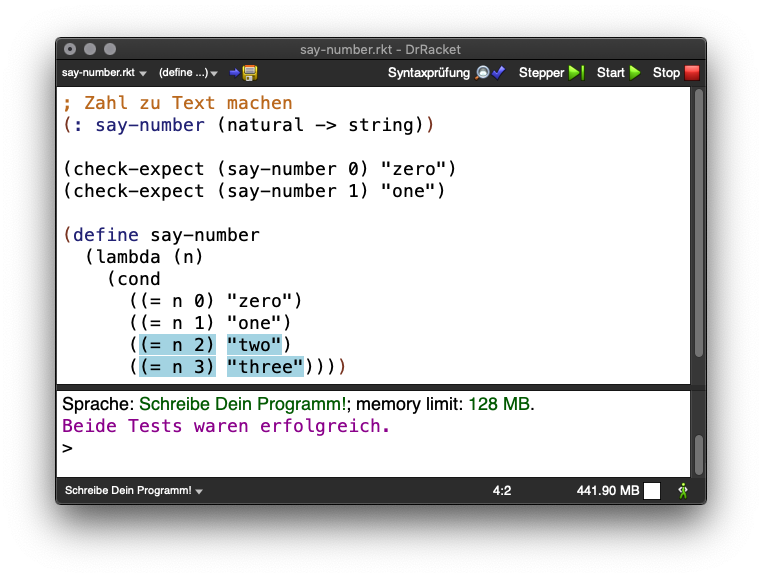
\includegraphics[width=0.7\textwidth]{fallunterscheidungen/coverage}
  \caption{Anzeige von Abdeckung in DrRacket}
  \label{fig:coverage}
\end{figure}

Vielleicht ist Dir bei der \lstinline{say-number}-Funktion aus dem
vorigen Abschnitt aufgefallen, dass bei dem Programm unmittelbar, nachdem
es gelaufen ist, zwei Zeilen farbig
hinterlegt sind, wie in Abbildung~\ref{fig:coverage} zu sehen.  Das liegt
daran, dass diese beiden Zeilen nie ausgewertet wurden, weil die
Tests nur die ersten beiden Fälle überprüfen.  Theoretisch
könnte in den beiden letzten Zweigen für $2$ und $3$ noch ein Fehler
stecken, und die Tests würden es nicht bemerken.

Wenn Du folgende Testfälle hinzufügst, geht die farbige Hinterlegung weg:
%
\begin{lstlisting}
(check-expect (say-number 2) "two")
(check-expect (say-number 3) "three")
\end{lstlisting}
%
Probier es aus~-- am besten erst nur den einen, dann den anderen!

Die farbige Hinterlegung zeigt die \textit{Abdeckung} an, wie wir es
schon in Abschnitt~\ref{page:abdeckung0} auf
Seite~\pageref{page:abdeckung0} kurz diskutiert haben: Ein Ausdruck im
Programm, der durch die Tests ausgewertet wird, heißt
\textit{abgedeckt}.  Die farbig hinterlegten Ausdrücke sind also nicht
abgedeckt.  Der letzte Satz von Konstruktionsanleitung~\ref{ka:tests}
auf Seite~\pageref{ka:tests} sagt genau das: Eine Funktion sollte
durch ihre Tests vollständig abgedeckt werden.  Die Abdeckung ist also
eine Minimalanforderung an unsere Tests.

\section{Aufzählungen}

\mentioncode{fallunterscheidungen/pet.rkt}
%
Nächste Beispielaufgabe: Wir wollen Haustiere einteilen in niedliche
und nicht so niedliche.  Es gibt in der Welt dieser Aufgabe nur drei
verschiedene Haustiere: Katzen, Hunde und Schlangen.  Haustiere
könnten wir in einem Kommentar im Programm so beschreiben:
%
\label{sec:datendefinition}
\begin{lstlisting}
; Ein Haustier ist eins der folgenden:
; - Katze
; - Hund
; - Schlange
\end{lstlisting}
%
Solch ein kurzer Kommentar, der die Daten beschreibt, die in unserer
Aufgabe vorkommen, heißt
\textit{Datendefinition\index{Datendefinition}}.  Mehr dazu in
Abschnitt~\ref{sec:datenanalyse}.  Die Formulierung der
Datendefinition "<eins der folgenden"> deutet daraufhin, dass auch
diese Sorte Daten in mehrere Fälle zerfällt~-- es handelt sich also
wieder um eine Fallunterscheidung.

Bevor wir die eigentliche Aufgabe lösen (niedlich oder nicht), müssen
wir uns zunächst überlegen, wie wir Haustiere im Programm
repräsentieren: Für die Zwecke dieser Aufgabe reicht es zu wissen, mit
\emph{welcher} der drei Möglichkeiten wir es zu tun haben.  Wir
benutzen die einfachste Möglichkeit, Zeichenketten mit dem
entsprechenden Text, also \lstinline{"Katze"}, \lstinline{"Hund"} und
\lstinline{"Schlange"}.

Eine solche Auflistung von Werten bildet eine sogenannte
\textit{Aufzählung\index{Aufzählung}}~-- ein Spezialfall einer
Fallunterscheidung.

Für die Aufzählung der Haustiere gibt es noch keine fertige Signatur,
die müssen wir noch definieren.  Die
\textit{Signatur-Definition\index{Signatur-Definition}} sieht so
aus:\indexvariable{pet}
\label{sec:pet}\label{page:signature}
%
\begin{lstlisting}
(define pet
  (signature (enum "Katze" "Hund" "Schlange")))
\end{lstlisting}
%
Da sind gleich zwei neue Programmelemente drin:
%
\begin{itemize}
\item Wir schreiben
  \lstinline{signature}\indexvariable{signature} immer, wenn wir eine
  neue Signatur erzeugen.
\item \lstinline{enum}\indexvariable{enum} (das funktioniert
  nur innerhalb eines \lstinline{signature}-Ausdrucks) ist für
  Aufzählungen zuständig.  In einem \lstinline{enum}-Ausdruck stehen
  die Werte, die zur Aufzählung gehören.
\end{itemize}
%
\begin{aufgabeinline}
  Die Funktion \lstinline{say-number} aus dem vorigen Abschnitt hat ja als
  Signatur-Deklaration die folgende:
\begin{lstlisting}
(: say-number ((integer-from-to 0 3) -> string))
\end{lstlisting}
  %
  Schreibe explizite Datendefinitionen für Ein- und Ausgabe der Funktion
  und mache ihre Signatur mit Hilfe von Aufzählungen präziser!
\end{aufgabeinline}
%
Zurück zu unserer Funktion zur Niedlichkeitsanalyse.  Die definierte
Signatur \lstinline{pet} können wir nun in der Signatur-Deklaration
unserer Funktion benutzen.  Zusammen mit der Kurzbeschreibung sieht
das so aus:
%
\begin{lstlisting}
; Ist Haustier niedlich?
(: cute? (pet -> boolean))
\end{lstlisting}
%
Das Fragezeichen gehört zum Namen der Funktion und ist eine
Konvention, die wir für die Namen von Funktionen verwenden, die einen
booleschen Wert zurückgeben~-- also solche Funktionen, die eine
Ja-/Nein-Frage beantworten.

Da es nur drei Möglichkeiten für die Eingabe gibt, können wir für alle
drei jeweils einen Test schreiben:
%
\begin{lstlisting}
(check-expect (cute? "Katze") #t)
(check-expect (cute? "Hund") #t)
(check-expect (cute? "Schlange") #f)
\end{lstlisting}
%
Kommen wir zur Funktion selbst.  Zunächst einmal das Gerüst:
%
\begin{lstlisting}
(define cute?
  (lambda (p)
    |\ldots|))
\end{lstlisting}
%
Da es sich bei der Eingabe um eine Aufzählung, also eine
Fallunterscheidung handel, brauchen wir eine Verzweigung im Rumpf.  Da
es drei Fälle in der Aufzählung gibt, braucht die Verzweigung
ebenfalls drei Zweige:
%
\begin{lstlisting}
(define cute?
  (lambda (p)
    (cond
      (|\ldots| |\ldots|)
      (|\ldots| |\ldots|)
      (|\ldots| |\ldots|))))
\end{lstlisting}
%
Als Nächstes müssen wir die Bedingungen schreiben, und die sollten
\lstinline{p} jeweils mit \lstinline{"Katze"}, \lstinline{"Hund"} und
\lstinline{"Schlange"} vergleichen.  Dabei könnte man leicht auf die Idee
kommen, \lstinline{(= p "Katze")} etc.\ zu schreiben.  Dann kommt
allerdings eine Fehlermeldung etwa so:
%
\begin{lstlisting}
=: Zahl als erstes Argument erwartet, "Katze" bekommen
\end{lstlisting}
%
Die Funktion \lstinline{=} fühlt sich also nur für Zahlen zuständig, für
Zeichenketten müssen wir die Funktion
\lstinline{string=?}\indexvariable{string=?} verwenden:
%
\begin{lstlisting}
(define cute?
  (lambda (p)
    (cond
      ((string=? p "Katze") |\ldots|)
      ((string=? p "Hund") |\ldots|)
      ((string=? p "Schlange") |\ldots|))))
\end{lstlisting}
%
Bisher ergibt sich alles rein aus der Definition von \lstinline{pet}.
Schließlich müssen wir noch die Antworten ergänzen.  Katzen und Hunde
sind niedlich, Schlangen nicht:
%
\indexvariable{cute?}
\begin{lstlisting}
(define cute?
  (lambda (p)
    (cond
      ((string=? p "Katze") #t)
      ((string=? p "Hund") #t)
      ((string=? p "Schlange") #f))))
\end{lstlisting}
%
Fertig!

\section{Zahlenbereiche}
\label{sec:zahlenbereiche}
\label{sec:heat-water}

\mentioncode{fallunterscheidungen/heat-water.rkt}
%
Eine weitere häufig vorkommende Art der Fallunterscheidung gibt es bei
Zahlenbereichen.

Um das zu demonstrieren, nehmen wir uns folgende Aufgabe vor: Wir
schreiben eine Funktion, die "<Wasser erhitzt">.
Das heißt, wir fügen einer bestimmten Menge Wasser bei einer
bestimmten Temperatur eine bestimmte Menge Wärme zu.  Wir wollen
berechnen, wie warm das Wasser danach ist.  Der Einfachheit halber
messen wir die zugefügte Wärme~-- genau wie die Temperatur~-- in Grad
Celsius (\si{\degree}C).\footnote{Wir vereinfachen schon sehr stark, aber 
  Temperaturerhöhung und Wärme sind über die Wärmekapazität verwandt.}
Wir schreiben dazu drei Versionen der
Funktion:
%
\begin{itemize}
\item Die erste, naive Version addiert einfach auf die
  Anfangstemperatur die hinzugefügte Wärme.
\item Die zweite Version berücksichtigt, dass Wasser bei 100\si{\degree}C siedet
  und nicht heißer werden kann.
\item Die dritte Version berücksichtigt zusätzlich, dass gefrorenem
  Wasser von 0\si{\degree}C eine Wärme von 80\si{\degree}C hinzugefügt werden muss, damit es
  schmilzt und dann immer noch erst bei 0\si{\degree}C ist.
\end{itemize}
%
Wir berücksichtigen also schrittweise, dass die innere Energie des
Wassers~-- die Wärme~-- nicht dasselbe ist wie dessen Temperatur.

\paragraph{Naive Version} Wir fangen mit der naiven Version an und gehen nach dem Ablauf der
Konstruktionsanleitungen vor.  Zuerst kommt also eine
Kurzbeschreibung:
%
\begin{lstlisting}
; Wassertemperatur nach Erhitzen berechnen, naiv
\end{lstlisting}
%
Als Nächstes kommt die Signatur-Deklaration.  Die Anfangstemperatur
und die hinzugefügte Wärme sind die Eingaben; sie stellen wir als
reelle Zahlen dar.  Heraus kommt die Endtemperatur, auch eine reelle
Zahl.  Da wir schon wissen, dass diese Version etwas einfach ist,
hängen wir eine \lstinline{-0} an den Namen:
%
\begin{lstlisting}
(: heat-water-0 (real real -> real))
\end{lstlisting}                
%
Nun schreiben wir einige einfache Beispiele als Testfälle hin:
%
\begin{lstlisting}
(check-expect (heat-water-0 -10 20) 10)
(check-expect (heat-water-0 10 20) 30)
(check-expect (heat-water-0 90 20) 110)
\end{lstlisting}
%
Als Nächstes kommt das Gerüst an die Reihe:
%
\begin{lstlisting}
(define heat-water-0
  (lambda (temp heat)
    |\ldots|))
\end{lstlisting}
%
Der Rumpf ist jetzt kein Hexenwerk, die beiden Eingaben werden
einfach addiert:
%
\indexvariable{heat-water-0}
\begin{lstlisting}
(define heat-water-0
  (lambda (temp heat)
    (+ temp heat)))
\end{lstlisting}
%
Noch die Tests laufen lassen und fertig!

\paragraph{Siedendes Wasser} Als Nächstes wollten wir berücksichtigen,
dass Wasser bei normalen Druckverhältnissen nicht über 100\si{\degree}C heiß werden kann.  Die Kurzbeschreibung
passen wir nur leicht an; die Signatur bleibt ebenfalls fast
unverändert~-- wir ändern nur den Namen und machen aus der $0$ eine $1$:
%
\begin{lstlisting}
; Wassertemperatur nach Erhitzen berechnen, Sieden berücksichtigen
(: heat-water-1 (real real -> real))
\end{lstlisting}
%
Bei den Tests können wir natürlich die Tests von \lstinline{heat-water-0}
kopieren, aber den letzten müssen wir anpassen:
%
\begin{lstlisting}
(check-expect (heat-water-1 -10 20) 10)
(check-expect (heat-water-1 10 20) 30)
(check-expect (heat-water-1 90 20) 100)
\end{lstlisting}
%
Beim Testen ist es immer sinnvoll, auch Grenzfälle zu testen~--
schaltet die Funktion wirklich um, wenn die 100 erreicht sind. %%Nicht rum!
                              
Dazu dienen folgende zwei Testfälle:
%
\begin{lstlisting}
(check-expect (heat-water-1 99 1) 100)
(check-expect (heat-water-1 99 2) 100)
\end{lstlisting}
%
Da die Signatur die gleiche ist, ist auch das Gerüst identisch:
%
\begin{lstlisting}
(define heat-water-1
  (lambda (temp heat)
    |\ldots|))
\end{lstlisting}
%
Ab 100\si{\degree}C muss die Funktion ihr Ergebnis also anders berechnen.  Oder,
anders gesagt, die Eingaben fallen in zwei verschiedene Klassen: die,
bei denen die Summe unter 100 liegt und die, bei denen sie darüber
liegt.
Wir benötigen also ein \lstinline{cond} mit zwei
Zweigen:
%
\begin{lstlisting}
(define heat-water-1
  (lambda (temp heat)
    (cond
      (|\ldots| |\ldots|)
      (|\ldots| |\ldots|))))
\end{lstlisting}
%
Wir brauchen nun eine Bedingung, die feststellt, ob die Summe aus
\lstinline{temp} und \lstinline{heat} unterhalb von 100 liegt (genauer:
kleiner \emph{oder gleich}, weil 100 gerade so erreichbar ist) und
eine dafür, dass die Summe darüber liegt.  Die könnten so aussehen:
%
\begin{lstlisting}
(<= (+ temp heat) 100)
(> (+ temp heat) 100)
\end{lstlisting}
%
Wenn wir diese beiden Bedingungen an die entsprechenden Stellen im
Rumpf setzen, sieht das so aus:
%
\begin{lstlisting}
(define heat-water-1
  (lambda (temp heat)
    (cond
      ((<= (+ temp heat) 100) |\ldots|)
      ((> (+ temp heat) 100) |\ldots|))))
\end{lstlisting}
%
An die Stellen nach den Bedingungen müssen wir Ausdrücke setzen, die
das Ergebnis liefern, das im jeweiligen Fall richtig ist.  Das wäre dann:
%
\indexvariable{heat-water-1}
\begin{lstlisting}
(define heat-water-1
  (lambda (temp heat)
    (cond
      ((<= (+ temp heat) 100) (+ temp heat))
      ((> (+ temp heat) 100) 100))))
\end{lstlisting}
%
Fertig!
%
%

%
\begin{aufgabeinline}
  Müssen es bei den beiden Bedingungen unbedingt \lstinline{<=} und
  \lstinline{>} sein?  Was passiert, wenn Du \lstinline{<=} durch \lstinline{<}
  ersetzt und das Programm dann laufen lässt?  Was passiert, wenn Du
  dann auch das \lstinline{>} ersetzt~-- durch \lstinline{>=}?  Warum
  funktioniert das Programm dann immer noch?
\end{aufgabeinline}
%
\paragraph{Siedendes Wasser und Eis} Kommen wir zur "<Vollversion">.
Zur Erinnerung: Da müssen wir noch berücksichtigen, dass gefrorenem
Wasser von 0\si{\degree}C eine Wärme von 80\si{\degree}C hinzugefügt werden muss, damit es
schmilzt und dann immer noch 0\si{\degree}C hat.  

Wir fangen wieder mit der Kurzbeschreibung an:
%
\begin{lstlisting}
; Wassertemperatur nach Erhitzen berechnen, mit Eis & Sieden
\end{lstlisting}
%
Da diese Version die letzte ist, hat sie keine Nummer mehr.  Ansonsten
ist die Signatur unverändert:
%
\begin{lstlisting}
(: heat-water (real real -> real))
\end{lstlisting}
%
Die Tests können wir nicht unverändert übernehmen.  Gleich der erste
funktioniert nicht mehr:
%
\begin{lstlisting}
(check-expect (heat-water -10 20) 10)
\end{lstlisting}
%
Das Aufwärmen des Wassers von $-10$\si{\degree}C auf $0$\si{\degree}C erfordert nur $10$\si{\degree}C
Wärmezufuhr, dann aber müssen erst einmal 80\si{\degree} weitere Wärme zugeführt
werden, damit es weiter geht.  Den Testfall müssen wir also ändern:
%
\begin{lstlisting}
(check-expect (heat-water -10 20) 0)
\end{lstlisting}
%
Die anderen Testfälle \lstinline{heat-water-1} können so bleiben:
%
\begin{lstlisting}
(check-expect (heat-water 10 20) 30)
(check-expect (heat-water 90 20) 100)
(check-expect (heat-water 99 1) 100)
(check-expect (heat-water 99 2) 100)
\end{lstlisting}
%
Ein paar weitere Tests sollten aber noch genau klären, was um den
Nullpunkt herum so passiert und wo genau er überschritten wird:
%
\begin{lstlisting}
(check-expect (heat-water -10 5) -5)
(check-expect (heat-water -5 60) 0)
(check-expect (heat-water -5 90) 5)
(check-expect (heat-water -1 81) 0)
(check-expect (heat-water -1 82) 1)
\end{lstlisting}
%
Wieder sollten wir darüber nachdenken, in welche Fälle unsere
Eingaben zerfallen.  Da gibt es drei naheliegende Fälle:
%
\begin{enumerate}
\item Die Anfangstemperatur ist unter $0$\si{\degree}C, es wird also Eis erwärmt.
\item Die Erwärmung würde die Wassertemperatur auf über $100$\si{\degree}C erhöhen.
\item Alles andere~-- das Wasser fängt flüssig an und bleibt durch die
  Erwärmung flüssig.
\end{enumerate}
%
Der erste Fall hat außerdem noch drei "<Unterfälle">:
%
\begin{itemize}
\item Die Erwärmumg bleibt unter $0$\si{\degree}C.
\item Die Erwärmung bleibt bei  $0$\si{\degree}C "<stecken">
\item Die Erwärmung erhöht die Temperatur über den Nullpunkt hinaus.
\end{itemize}
%
So komplizierte Fallunterscheidungen sind relativ selten. Wenn sie
doch einmal auftauchen, ist besondere Sorgfalt gefragt.  Deshalb
exerzieren wir das hier als Beispiel durch.

Fangen wir wieder mit dem Gerüst für die Funktion an:
%
\begin{lstlisting}
(define heat-water
  (lambda (temp heat)
    |\ldots|))
\end{lstlisting}
%
Wir wissen schon aus der Analyse der Fälle, dass es drei Fälle gibt.
Deshalb brauchen wir auch wieder ein \lstinline{cond} mit drei Zweigen.
%
\begin{lstlisting}
(define heat-water
  (lambda (temp heat)
    (cond
      (|\ldots| |\ldots|)
      (|\ldots| |\ldots|)
      (|\ldots| |\ldots|))))
\end{lstlisting}
%
Jetzt ergänzen wir Bedingungen, die den drei Fällen entsprechen.  Um
in diesem komplizierten Fall die Zuordnung von Fällen und Bedingungen
klar erkennbar zu machen, stehen diese jeweils als Kommentar darüber:
%
\begin{lstlisting}
(define heat-water
  (lambda (temp heat)
    (cond
      ; Die Anfangstemperatur ist unter 0|\si{\degree}|C, es wird also Eis erwärmt.
      ((< temp 0) |\ldots|)
      ; Erwärmung würde Wassertemperatur auf über 100|\si{\degree}|C erhöhen.
      ((>= (+ temp heat) 100) |\ldots|)
      ; Wasser fängt flüssig an und bleibt durch Erwärmung flüssig.
      ((and (>= temp 0) (< (+ temp heat) 100)) |\ldots|))))
\end{lstlisting}
%
Jetzt können wir uns daran machen, die Zweige auszufüllen.  Da der
erste Zweig (das Eis) komplizierter ist, schieben wir den erstmal vor
uns her.  Beim zweiten Zweig kommt einfach 100\si{\degree}C raus.  Ebenso
einfach ist der dritte Zweig, bei dem das Wasser flüssig bleibt~-- die
Antwort ist dort \mbox{\lstinline{(+ temp heat)}}.  Der Zwischenstand sieht so
aus:
%
\begin{lstlisting}
(define heat-water
  (lambda (temp heat)
    (cond
      ; Die Anfangstemperatur ist unter 0|\si{\degree}|C, es wird also Eis erwärmt.
      ((< temp 0) |\ldots|)
      ; Erwärmung würde Wassertemperatur auf über 100|\si{\degree}|C erhöhen.
      ((>= (+ temp heat) 100) 100)
      ; Wasser fängt flüssig an und bleibt durch Erwärmung flüssig.
      ((and (>= temp 0) (< (+ temp heat) 100))
       (+ temp heat)))))
\end{lstlisting}
%
Dass wir die leichten Fälle zuerst bearbeitet haben, mag wie Faulheit
aussehen.  Ist es auch~-- aber es ist auch eine sinnvolle Strategie, die
sich aus Mantra~\ref{mantra:schreib} ergibt:

\mantraschreib*
%
\noindent Auch über den ersten Zweig wissen wir etwas, nämlich dass er selbst
eine Fallunterscheidung ist mit drei Fällen.  Wir können also das
\lstinline{cond} (wieder einmal) schon hinschreiben:
%
\begin{lstlisting}
(define heat-water
  (lambda (temp heat)
    (cond
      ; Anfangstemperatur ist unter 0|\si{\degree}|C, es wird also Eis erwärmt.
      ((< temp 0)
       (cond
         (|\ldots| |\ldots|)
         (|\ldots| |\ldots|)
         (|\ldots| |\ldots|)))
      ; Erwärmung würde die Wassertemperatur auf über 100|\si{\degree}|C erhöhen.
      ((>= (+ temp heat) 100) 100)
      ; Wasser fängt flüssig an und bleibt durch Erwärmung flüssig.
      ((and (>= temp 0) (< (+ temp heat) 100))
       (+ temp heat)))))
\end{lstlisting}
%
Auch hier ist es sinnvoll, die Beschreibungen der Fälle über die
Zweige zu schreiben.  Danach ergänzen wir die Bedingungen mit
folgendem Ergebnis:
%
\begin{lstlisting}
(define heat-water
  (lambda (temp heat)
    (cond
      ; Anfangstemperatur ist unter 0|\si{\degree}|C, es wird also Eis erwärmt.
      ((< temp 0)
       (cond
         ; Erwärmumg bleibt unter 0|\si{\degree}|C.
         ((< (+ temp heat) 0)
          |\ldots|)
         ; Erwärmung bleibt bei  0|\si{\degree}|C "stecken".
         ((and (>= (+ temp heat) 0)
               (< (+ temp heat) 80))
          |\ldots|)
         ; Erwärmung erhöht Temperatur über den Nullpunkt hinaus.
         ((and (>= (+ temp heat) 0)
               (>= (+ temp heat) 80))
          |\ldots|)))
      ; Erwärmung würde Wassertemperatur auf über 100|\si{\degree}|C erhöhen.
      ((>= (+ temp heat) 100) 100)
      ; Wasser fängt flüssig an und bleibt durch Erwärmung flüssig.
      ((and (>= temp 0) (< (+ temp heat) 100))
       (+ temp heat)))))
\end{lstlisting}
%
Die Bedingungen sind jetzt noch komplizierter, aber erschließen sich
hoffentlich durch genauere Betrachtungen:
%
\begin{itemize}
\item "<Die Erwärmumg bleibt unter $0$\si{\degree}C.">\\
  Das heißt, die Summe von
  Anfangstemperatur und Erwärmung ist kleiner als $0$\si{\degree}C.
\item "<Die Erwärmung bleibt bei  0\si{\degree}C stecken.">\\
  In diesem Fall muss die Summe von Temperatur und Erwärmung zwischen $0$\si{\degree}C
  und $80$\si{\degree}C liegen.
\item "<Die Erwärmung erhöht die Temperatur über den Nullpunkt hinaus.">\\
  Das Summe von Temperatur und Erwärmung geht nicht nur über $0$\si{\degree}C
  sondern auch über 80\si{\degree}C hinaus.
\end{itemize}
%
Die Antworten unter diesen Bedingungen sind vergleichsweise einfach zu
ergänzen:
%
\begin{lstlisting}
(define heat-water
  (lambda (temp heat)
    (cond
      ; Anfangstemperatur ist unter 0|\si{\degree}|C, es wird also Eis erwärmt.
      ((< temp 0)
       (cond
         ; Erwärmumg bleibt unter 0|\si{\degree}|C.
         ((< (+ temp heat) 0)
          (+ temp heat))
         ; Erwärmung bleibt bei  0|\si{\degree}|C "stecken".
         ((and (>= (+ temp heat) 0)
               (< (+ temp heat) 80))
          0)
         ; Erwärmung erhöht Temperatur über den Nullpunkt hinaus.
         ((and (>= (+ temp heat) 0)
               (>= (+ temp heat) 80))
          (- (+ temp heat) 80))))
      ; Erwärmung würde Wassertemperatur auf über 100|\si{\degree}|C erhöhen.
      ((>= (+ temp heat) 100) 100)
      ; Wasser fängt flüssig an und bleibt durch Erwärmung flüssig.
      ((and (>= temp 0) (< (+ temp heat) 100))
       (+ temp heat)))))
\end{lstlisting}
%
Fertig!\footnote{Allerdings noch nicht ganz richtig: Vielleicht siehst Du,
  dass da noch etwas nicht ganz stimmt.  Wir kommen später darauf zurück.}

\medskip

Also \emph{fast} fertig.  Wenn wir das Programm näher betrachten,
fällt etwas Verbesserungspotenzial auf.  Fangen wir an mit der
Bedingung:
%
\begin{lstlisting}
          (and (>= (+ temp heat) 0)
               (>= (+ temp heat) 80))
\end{lstlisting}
%
Eine Temperatur über 80\si{\degree}C liegt auch über 0\si{\degree}C.
Wir können das also vereinfachen zu:
%
\begin{lstlisting}
          (>= (+ temp heat) 80)
\end{lstlisting}
%
Das ist mathematisch einleuchtend, zur Sicherheit sollten wir aber die
Tests nochmals laufen lassen: Aber sie laufen alle noch erfolgreich
durch.

Bevor wir die Funktion noch weiter vereinfachen, ist es sinnvoll, die
Funktionsweise der Auswertung von \lstinline{cond}-Ausdrücken zu ergründen:
%
\begin{aufgabeinline}
  Lasse die \lstinline{heat-water}-Funktion im Stepper laufen und
  beobachte, wie~-- vor allem in welcher Reihenfolge~-- die Bedindungen
  in einem \lstinline{cond}-Ausdruck ausgewertet werden.
\end{aufgabeinline}
%
Wenn Du diese Aufgabe erledigt hast, wirst Du beobachtet haben, dass DrRacket
die Bedingungen in einem \lstinline{cond}-Ausdruck nacheinander
auswertet.  Sobald eine davon \lstinline{#t} ergibt, macht DrRacket mit dem
Ausdruck dieses Zweiges weiter.  Die restlichen Zweige werden gar nicht
mehr berücksichtigt, unabhängig davon, ob sie \lstinline{#t} ergeben
könnten.
Das können wir ausnutzen, um die Funktion weiter zu vereinfachen.
Wir betrachten die ersten beiden Bedingungen im "<inneren">
\lstinline{cond}:
%
\begin{lstlisting}
       (cond
         ((< (+ temp heat) 0) (+ temp heat))
         ((and (>= (+ temp heat) 0)
               (< (+ temp heat) 80))
          0)
         |\ldots|)
\end{lstlisting}
%
Wenn die erste Bedingung in diesem Ausschnitt \lstinline{#f} ergeben hat, also nicht stimmt,
dann ist \lstinline{(+ temp heat)} größer oder gleich 0.  Das heißt, der
Teilausdruck \lstinline{(>= (+ temp heat) 0)} in der \emph{nächsten}
Bedingung liefert \emph{immer} \lstinline{#t}.  Wir können also
vereinfachen:
%
\begin{lstlisting}
       (cond
         ((< (+ temp heat) 0) (+ temp heat))
         ((and #t
               (< (+ temp heat) 80))
          0)
         |\ldots|)
\end{lstlisting}
%
Ein Ausdruck \lstinline{(and #t $e$)} liefert immer das gleiche Ergebnis
wie \(e\)~-- schau nochmal auf Seite~\pageref{page:and}, um Dich davon
zu überzeugen!  Wir können also das innere \lstinline{cond} weiter
vereinfachen zu:

\begin{lstlisting}
       (cond
         ((< (+ temp heat) 0) (+ temp heat))
         ((< (+ temp heat) 80) 0)
         |\ldots|)
\end{lstlisting}
%
\label{page:bedingungen-vereinfachen}
Wir benutzen also Mathematik (genauer gesagt
\textit{Algebra\index{Algebra}}, also die Lehre der Gleichungen), um
unser Programm zu vereinfachen.  Algebra ist ein sehr mächtiges
Werkzeug in der Programmierung, und wir werden es noch oft nutzen.
Das fällt oft einfacher, wenn wir gar nicht über die konkrete
Bedeutung der Ausdrücke nachdenken sondern nur Gleichungen benutzen,
wie oft in der Mathematik und entsprechend
Mantra~\ref{mantra:gleichungen} auf Seite~\pageref{mantra:gleichungen}.

Wir sind aber mit dem Vereinfachen noch nicht fertig. Betrachten wir
nun die drei "<äußeren"> Bedingungen:
%
\begin{lstlisting}
    (cond
      ((< temp 0) |\ldots|)
      ((>= (+ temp heat) 100) |\ldots|)
      ((and (>= temp 0) (< (+ temp heat) 100)) |\ldots|))
\end{lstlisting}
%
Wenn die erste Bedingungen \lstinline{#f} ergibt, gilt automatisch
\lstinline{(>= temp 0)}.  Wir können die letzte Bedingung also
vereinfachen zu:
%
\begin{lstlisting}
(and #t (< (+ temp heat) 100))
\end{lstlisting}
%
Wenn auch die zweite Bedingung \lstinline{#f} ergibt, gilt auch
\lstinline{(< (+ temp heat) 100)}.
Wir können also vereinfachen zu \lstinline{(and #t #t)}
und von da zu \lstinline{#t}.

Wir können die Funktion mit dieser Einsicht vereinfachen und \lstinline{#t}
als Bedingung hinschreiben.  (Probier es aus!)  Allerdings finden
manche das hässlich: Darum ist es auch möglich, statt \lstinline{#t} das
besondere Wort \lstinline{else}\indexvariable{else}
("<andernfalls"> auf Englisch) hinzuschreiben.
Der \lstinline{else}-Zweig kommt also zum Zug, wenn alle anderen
"<durchgefallen"> sind.  Das Ergebnis sieht
dann so aus:
%
\indexvariable{heat-water}
\begin{lstlisting}
(define heat-water
  (lambda (temp heat)
    (cond
      ; Anfangstemperatur ist unter 0|\si{\degree}|C, es wird also Eis erwärmt.
      ((< temp 0)
       (cond
         ; Erwärmumg bleibt unter 0|\si{\degree}|C.
         ((< (+ temp heat) 0) (+ temp heat))
         ; Erwärmung bleibt bei  0|\si{\degree}|C "stecken".
         ((< (+ temp heat) 80) 0)
         ; Erwärmung erhöht Temperatur über den Nullpunkt hinaus.
         (else (- (+ temp heat) 80))))
      ; Erwärmung würde Wassertemperatur auf über 100|\si{\degree}|C erhöhen.
      ((>= (+ temp heat) 100) 100)
      ; Wasser fängt flüssig an und bleibt durch Erwärmung flüssig.
      (else
       (+ temp heat)))))
\end{lstlisting}
%
\begin{feature}{Verzweigung}{scheme:cond}
In den Lehrsprachen werden Verzweigungen\index{Verzweigung}\index{Verzweigung}
mit der Spezialform \lstinline{cond}\indexvariable{cond} dargestellt.
Ein \lstinline{cond}"=Ausdruck hat die folgende Form:
%
\begin{lstlisting}
(cond
  (|\(b\sb{1}\)| |\(a\sb{1}\)|)
  (|\(b\sb{2}\)| |\(a\sb{2}\)|)
  |\(\ldots\)|
  (|\(b\sb{n-1}\)| |\(a\sb{n-1}\)|)
  (else |\(a\sb{n}\)|))
\end{lstlisting}
%
Dabei sind die $b_i$ und die $a_i$ ihrerseits Ausdrücke.  Der
\lstinline{cond}-Ausdruck wertet nacheinander alle Bedingungen $b_i$ aus;
sobald eine Bedingung $b_k$ \lstinline{#t} ergibt, wird der
\lstinline{cond}-Ausdruck durch das entsprechende $a_k$ ersetzt.  Wenn
alle Bedingungen fehlschlagen, wird durch $a_n$ ersetzt.  Die Paarungen
\lstinline{($b_i$ $a_i$)} heißen \textit{Zweige\index{Zweig}} des
\lstinline{cond}-Ausdruckes, und der Zweig mit \lstinline{else}  heißt
\textit{\lstinline{else}-Zweig\index{else-Zweig@\texttt{else}-Zweig}}.
Der \lstinline{else}-Zweig kann auch fehlen~-- dann sollte aber immer
eine der Bedingungen  \lstinline{#t} ergeben.  Wenn doch einmal bei allen
$b_i$ \lstinline{#f} herauskommen sollte, bricht \drscheme{} das Programm ab
und gibt eine Fehlermeldung aus.
\end{feature}
%
Damit haben wir die komplette Funktionsweise von \lstinline{cond}
angewendet. Abbildung~\ref{scheme:cond} fasst sie noch einmal zusammen.

Du kannst von vornherein \lstinline{else} benutzen, wenn Du Dir
sicher bist, dass alle anderen Fälle schon in den vorigen Zweigen
abgedeckt sind.  Im Zweifelsfall empfehlen wir aber immer den Weg über
die Mathematik, damit die Funktion auch korrekt wird.

Apropos korrekt: Ist \lstinline{heat-water} korrekt?  Hier ist ein
weiterer Testfall:
%
\begin{lstlisting}
(check-expect (heat-water -1 191) 100)
\end{lstlisting}
%
Von den 191\si{\degree}C wird 1\si{\degree}C benötigt, um auf 0\si{\degree}C zu kommen, dann weitere
80\si{\degree}C, um über 0\si{\degree}C hinauszukommen, bleiben 110\si{\degree}C.  Aber über 100\si{\degree}C geht
es natürlich trotzdem nicht.  Leider sieht die Funktion das anders:
%
\begin{alltt}
Check-Fehler:
	Der tatsächliche Wert 110 ist nicht der erwartete Wert 100.
\end{alltt}
%
Woran liegt das?  Wenn wir die Verzweigungen im Kopf nachvollziehen,
sehen wir, dass zunächst der erste Zweig des äußeren \lstinline{cond}
greift, weil die Bedingung \lstinline{(< temp 0)} als Wert \lstinline{#t} hat.
Im inneren \lstinline{cond} schließlich ergeben die ersten beiden
Bedingungen jeweils \lstinline{#f}, es bleibt also der \lstinline{else}-Zweig,
und addiert die Wärme "<blind"> auf die Anfangstemperatur.

Wir müssen also unser Programm korrigieren, weil dieser Fall noch
nicht berücksichtigt ist: Die Anfangstemperatur ist unter 0\si{\degree}C, die
Erwärmung würde die Temperatur aber über 100\si{\degree}C heben.  Es greift also
der \lstinline{else}-Zweig des inneren \lstinline{cond} des äußeren Zweigs
mit \lstinline{(< temp 0)}, und das ist in diesem Fall falsch.  Die
ersten beiden Zweige sind für Endtemperaturen bis 0\si{\degree}C zuständig, wir
müssen also den neuen Zweig unmittelbar vor dem \lstinline{else}-Zweig
einfügen.  Der sieht so aus:
%
\begin{lstlisting}
         ; Erwärmung würde die Temperatur auf über 100|\si{\degree}|C bringen
         ((>= (- (+ temp heat) 80) 100) 100)
\end{lstlisting}
%
Jetzt ist das Programm endlich fertig und korrekt!

Doch wie konnte dieser Fehler unbemerkt bleiben, zumindest zunächst
von uns?  Das liegt daran, dass die Fallunterscheidung, die der
Aufgabe zugrundliegt, ziemlich komplex ist.  Bei komplexen Programmen
ist das Risiko \emph{immer} groß, dass sie Fehler enthalten.  Bei
komplexen Fallunterscheidungen bedeutet dies, dass fast immer ein Fall
im Programm fehlt, zumindest beim ersten Anlauf.  Wir sollten uns bei
der Gelegenheit an Mantra~\ref{mantra:komplexitaet} auf
Seite~\pageref{mantra:komplexitaet} erinnern:

\mantrakomplexitaet*

\noindent Bei komplizierten Fallunterscheidungen, teste deshalb gründlich und
gehe davon aus, dass Du Zweige vergessen hast.

\paragraph{Einfacher Wasser erhitzen}

Aus Mantra~\ref{mantra:komplexitaet} kann man auch noch eine und
bessere Schlussfolgerung ziehen, als einfach nur sorgfältig zu prüfen
und zu testen.  Wenn nämlich die Fallunterscheidungen so kompliziert
sind, dann solltest Du gründlich prüfen, ob es nicht auch einfacher
geht.

Wir haben dieses Prinzip beim Schreiben dieses Buchs leider
vernachlässigt.  Glücklicherweise hat Nicolas Neuß von der Universität
Erlangen eine Vorabversion dieses Buches gelesen.  Ihm stieß die
Komplexität der Funktion ebenfalls auf, und er machte folgenden
Vorschlag:
%
\begin{quote}
  Das Ganze wird meiner Meinung nach viel hübscher, wenn man das
  physikalischer angeht.  Wenn man daher Konversionsroutinen
  \verb|E->T| und \verb|T->E| schreibt (\texttt{E} steht für innere
  Energie, also die Wärme, und \texttt{T} für Temperatur), so sieht
  man erstens die Problematik und zweitens kann man die
  Temperaturerhöhung einfach berechnen.
\end{quote}
%
Wir versuchen mal, Dr.\ Neuß' Idee nachzuvollziehen.  Wir fangen mit
der von ihm erwähnten Funktion \verb|E->T| an.  In unserer
Terminologie könnte die Funktion \lstinline{heat->temperature} heißen,
mit folgender Kurzbeschreibung und Signatur:
%
\begin{lstlisting}
; Aus Wärme Temperatur berechnen
(: heat->temperature (real -> real))
\end{lstlisting}
%
Entsprechend den Ausführungen am Anfang des Abschnitts entsprechen
unterhalb von 0\si{\degree}C die Temperatur und die Wärme einander.  Bei Wärme
zwischen 0\si{\degree}C und 80\si{\degree}C ist die Temperatur konstant 0\si{\degree}C. Ab 80\si{\degree}C Wärme
führt jedes Grad Erhöhung auch zu einer Erhöhung der Temperatur, bis
100\si{\degree}C Temperatur beziehungsweise 180\si{\degree}C Wärme erreicht sind.  Ab da
bleibt die Temperatur bei 100\si{\degree}C, auch wenn die Wärme steigt.

Die Testfälle dazu könnten also so aussehen:
%
\begin{lstlisting}
(check-expect (heat->temperature -50) -50)
(check-expect (heat->temperature 0) 0)
(check-expect (heat->temperature 20) 0)
(check-expect (heat->temperature 80) 0)
(check-expect (heat->temperature 81) 1)
(check-expect (heat->temperature 180) 100)
(check-expect (heat->temperature 200) 100)                                            
\end{lstlisting}
%
Die Eingabe-Wärme zerfällt entsprechend der Beschreibung oben in vier
Fälle, die wir als vier Zweige eines \lstinline{cond} schreiben:
%
\begin{lstlisting}
(define heat->temperature
  (lambda (heat)
    (cond
      (... ...)
      (... ...)
      (... ...)
      (... ...))))
\end{lstlisting}
%
Die Bedingungen und Ausdrücke ergeben sich direkt aus der Beschreibung:
%
\indexvariable{heat->temperature}
\begin{lstlisting}
(define heat->temperature
  (lambda (heat)
    (cond
      ((<= heat 0) heat)
      ((and (< 0 heat)
            (<= heat 80))
       0)
      ((and (< 80 heat)
            (<= heat 180))
       (- heat 80))
      ((< 180 heat) 100))))
\end{lstlisting}
%
Wir brauchen noch eine Funktion in die andere Richtung, die
wir \lstinline{temperature->heat} nennen. Diese Funktion ist einfacher:
Temperaturen bis 0\si{\degree}C entsprechen der Wärme, Temperaturen darüber
brauchen 80\si{\degree}C mehr Wärme.  Es gibt also nur zwei Fälle und damit zwei
Zweige:
%
\indexvariable{temperature->heat}
\begin{lstlisting}
; Aus Temperatur Wärme berechnen
(: temperature->heat (real -> real))

(check-expect (temperature->heat -20) -20)
(check-expect (temperature->heat -1) -1)
(check-expect (temperature->heat 1) 81)
(check-expect (temperature->heat 100) 180)

(define temperature->heat
  (lambda (temp)
    (cond
      ((< temp 0) temp)
      ((and (> temp 0)
            (<= temp 100))
       (+ temp 80)))))
\end{lstlisting}
%
Dr.\ Neuß schlug vor, diese beiden Funktionen dazu zu benutzen, um den
Rumpf von \lstinline{heat-water} zu schreiben.  Wir versuchen das
und schreiben eine neue Funktion
\lstinline{heat-water-2}, bevor wir die alte wegwerfen:
%
\indexvariable{heat-water-2}
\begin{lstlisting}
; Wassertemperatur nach Erhitzen berechnen, mit Eis & Sieden
(: heat-water-2 (real real -> real))

(define heat-water-2
  (lambda (temp heat)
    ...))
\end{lstlisting}
%
(Wir nehmen die gleichen Testfälle wie bei \lstinline{heat-water}.)
Wie können wir \lstinline{heat->temperature} und
\lstinline{temperature->heat} einbringen?  Nun, wir können für
\lstinline{temp} die zugehörige Wärme berechnen, \lstinline{heat}
addieren, und das Ganze wieder zurück in eine Temperatur wandeln:
%
\indexvariable{heat-water-2}
\begin{lstlisting}
(define heat-water-2
  (lambda (temp heat)
    (heat->temperature
     (+ (temperature->heat temp) heat))))
\end{lstlisting}
%
Die Funktion besteht alle Testfälle.  Besser noch, die
beiden Funktionen \lstinline{heat->temperature} und
\lstinline{temperature->heat} sind viel einfacher zu verstehen als der
Moloch \lstinline{heat-water}.

Bei komplizierten Verzweigungen~-- generell bei allen komplizierten
Programmen~-- ist es wert zu untersuchen, ob es auch einfacher geht.

\section{Datenanalyse und Schablonen}
\label{sec:datenanalyse}

In Abschnitt~\ref{sec:datendefinition} auf
Seite~\pageref{sec:datendefinition} ist zum ersten Mal eine
\textit{Datendefinition\index{Datendefinition}} aufgetaucht:
%
\begin{lstlisting}
; Ein Haustier ist eins der folgenden:
; - Katze
; - Hund
; - Schlange
\end{lstlisting}
%
Diese Datendefinition ist das Ergebnis eines Nachdenkprozesses, der
sogenannten \textit{Datenanalyse\index{Datenanalyse}}.  Dieser Begriff
ist schon in Abschnitt~\ref{sec:konstruktionsanleitungen} auf
Seite~\pageref{sec:konstruktionsanleitungen} aufgetaucht, als zweiter
Schritt der Konstruktionsanleitung: Ab sofort werden wir diesen
Schritt immer durchführen, weil er zentral ist für die systematische
Konstruktion von Programmen.

Die Vorgehensweise bei einer Datenanalyse sieht im Allgemeinen so aus:
%
\begin{konstruktionsanleitung}{Datenanalyse}
  Suche in der Aufgabenstellung nach problemrelevanten Größen;
  Kandidaten sind immer die Substantive. Schreibe für jede dieser
  Größen eine Datendefinition, es sei denn, diese ist aus dem Kontext
  offensichtlich.

  Wenn es für die Datendefinition noch keine Signatur gibt, schreibe
  eine Signatur-Definition dazu.  Schreibe außerdem Beispiele auf und
  schreibe jeweils einen Kommentar, der die Beziehung zwischen Daten
  und Information beschreibt.
\end{konstruktionsanleitung}
%
\emph{Wie} Du die Signatur-Definition schreibst, dafür gibt es in
diesem Buch eine Reihe spezialisierter Konstruktionsanleitungen.  Die
Beziehung zwischen Daten und Information geht auf
Abschnitt~\ref{sec:information-daten} auf
Seite~\pageref{sec:information-daten} zurück.

In diesem Fall ist "<Haustier"> eine problemrelevante Größe, zu der
wir eine Datendefinition geschrieben haben.  Bei der Erwärmung von
Wasser haben wir allerdings nicht extra hingeschrieben, dass die
Wassertemperatur eine reelle Zahl ist, weil dies allgemein bekannt
ist.

Für die Formulierung der Datendefinition gibt es eine Reihe von
typischen Mustern, die sich immer wiederfinden.  Eines ist bei der
Definition von "<Haustier"> ersichtlich, nämlich "<eins der
folgenden">, das darauf hinweist, dass es sich bei "<Haustier"> um
eine Fallunterscheidung handelt.  

\begin{konstruktionsanleitung}{Fallunterscheidung: Datenanalyse}
  \label{ka:fallunterscheidung}
  Versuche, für die Datendefinition eine Formulierung "<\ldots{}
    ist eins der folgenden"> zu finden. Wenn das möglich ist, beschreibt
  Deine Datendefinition eine
  \textit{Fallunterscheidung\index{Fallunterscheidung}}.  Schreibe
  dann eine Auflistung aller Fälle, jeder Fall auf eine separate
  Zeile:
  
\begin{lstlisting}
; Ein X ist eins der folgenden:
; - Fall 1
; - Fall 2
; - ...
; - Fall n
\end{lstlisting}
\end{konstruktionsanleitung}
%
Für den Sonderfall der Aufzählung haben wir folgende Konstruktionsanleitung:
%
\begin{konstruktionsanleitung}{Aufzählung: Datenanalyse}
  \label{ka:aufzaehlung}
  Falls Deine Datendefinition eine Fallunterscheidung beschreibt und
  jeder der Fälle nur aus einem einzelnen Wert besteht, handelt es
  sich um eine \textit{Aufzählung\index{Aufzählung}}.

  Schreibe für jede Aufzählung eine Signatur-Definition der Form:
  % 
\begin{lstlisting}
(define |\(s\)| (signature (enum |\ldots|)))
\end{lstlisting}
  %
  Achte darauf, dass die Anzahl der Fälle der Signatur-Definition der
  Anzahl der Fälle der Datendefinition entspricht.
\end{konstruktionsanleitung}
%
Die Datenanalyse ist die wichtigste Methode zur Umsetzung der
Mantras~\ref{mantra:schreib} und \ref{mantra:lies}:
%
\mantraschreib*
%
\mantralies*
%
\noindent Die Datenanalyse lenkt zunächst den Blick auf die
Daten, \emph{nicht} darauf, was mit ihnen gemacht wird.  (Das
kommt später.)  Außerdem führt sie immer zu Elementen in unserem Programm.
Bei der Funktion \lstinline{cute?} haben wir aus der
Datendefinition zunächst eine Signatur-Definition abgeleitet:
%
\indexvariable{pet}
\begin{lstlisting}
(define pet
  (signature (enum "Katze" "Hund" "Schlange")))
\end{lstlisting}
%
Bei Aufzählungen stehen alle Beispiele schon in der
Signatur-Definition.  Wir müssen deshalb nicht noch separat
Beispiele aufschreiben.

Da die Datendefinition für "<Haustier"> drei Fälle hat, muss auch die
Signatur-Definition drei Fälle haben.  Aus der Signatur-Definition
ergibt sich direkt eine Verzweigung im Rumpf, die sich nur aus der
Signatur \lstinline{(pet -> boolean)} beziehungsweise der
Signatur-Definition von \lstinline{pet} als Aufzählung mit drei Fällen
ergibt:
%
\indexvariable{cute?}
\begin{lstlisting}
(define cute?
  (lambda (p)
    (cond
      (|\ldots| |\ldots|)
      (|\ldots| |\ldots|)
      (|\ldots| |\ldots|))))
\end{lstlisting}
%
Da \lstinline{cute?} eine Eingabe zur Signatur \lstinline{pet} erwartet und
\lstinline{pet} eine Aufzählungssignatur mit \emph{drei} Fällen ist, \emph{muss}
im Rumpf eine Verzweigung mit ihrerseits \emph{drei} Zweigen
auftauchen, ganz egal, was die konkrete Aufgabenstellung ist.  Wir
betonen das Wort \emph{drei} deshalb so, weil viele Fehler dadurch
passieren, dass die Anzahl der Zweige im \lstinline{cond} einer solchen
Funktion nicht der Anzahl der Fälle entspricht.

So ein unfertiges Programm, in dem sich einige Elemente aus der
Analyse der Daten ergeben haben ohne besondere Berücksichtigung der
konkreten Aufgabenstellung, heißt \textit{Schablone}.  Zu bestimmten
Arten von Datendefinitionen gehören bestimmte Schablonen.

\begin{konstruktionsanleitung}{Schablone}
  \index{Schablone}
  Wenn Du das Gerüst fertiggestellt hast, benutze die Signatur und die
  dazugehörigen Datendefinitionen, um Konstruktionsanleitungen mit ein
  oder mehreren Schablonen auszuwählen und übertrage die Elemente der
  Schablonen in den Rumpf der Funktion.
\end{konstruktionsanleitung}
%
Die Schablone ist das nächste Werkzeug für die Umsetzung von
Mantra~\ref{mantra:schreib}:
%
\mantraschreib*
%
\noindent Für jede Sorte von Datendefinition schreiben wir neben der
Konstruktionsanleitung für die Datenanalyse auch eine für die
Schablone.  Hier die Schablone für Fallunterscheidungen:
%
\begin{konstruktionsanleitung}{Fallunterscheidung: Schablone}
  \label{ka:fallunterscheidung-schablone}
  Wenn Du eine Funktion schreibst, die eine Fallunterscheidung als
  Eingabe verarbeitet, schreibe als Schablone in den Rumpf eine
  Verzweigung mit so vielen Zweigen, wie es in der Fallunterscheidung
  Fälle gibt, nach folgendem Muster:
  %
\begin{lstlisting}
(define |\(f\)|
  (lambda (|\(a\)|)
    (cond
      (|\ldots| |\ldots|)
      |\ldots|
      (|\ldots| |\ldots|))))
\end{lstlisting}
  Schreibe danach Bedingungen in die Zweige, welche die einzelnen
  Fälle voneinander unterscheiden.
\end{konstruktionsanleitung}
%
Diese Konstruktionsanleitung mag Dir ziemlich bürokratisch vorkommen,
und das ist sie auch.  Es mag Dir langweilig vorkommen, sie stur zu
befolgen, und das ist bestimmt ab und zu der Fall.  Dafür nehmen die
Konstruktionsanleitungen Dir viel Denkarbeit ab, und Du kannst Dein
Gehirn dann für die Lösung der eigentlichen Problemstellung verwenden,
wenn erst einmal die Schablone steht.  Spätestens also wenn Du vor
einer vermeintlich schweren Aufgabe stehst, wende erst einmal die
Konstruktionsanleitungen an, bevor Du Dir Sorgen machst, ob am Ende
alles aufgeht.  Was am Ende übrigbleibt, ist oft erstaunlich einfach.

\section{Exkurs: Verzweigungen in der Mathematik}

In der Mathematik gibt es auch Verzweigungen.  Diese werden in der
Regel mit einer großen geschweiften Klammer geschrieben.  In der
Mathematik ist es allerdings üblich, alle Bedingungen
"<auszuschreiben">, also ihre Bedeutung nicht von der Reihenfolge der
Auswertung abhängig zu machen, wie wir es bei \lstinline{heat-water}
getan haben.  Die Funktion schreiben wir den mathematischen
Gepflogenheiten entsprechend als einbuchstabige Funktion $h$ mit
Parametern $t$ für \lstinline{temp} und $h$ für \lstinline{heat}.  Das
$\deq$\index{*@$\deq$} steht für "<ist definiert als"> und das
mathematische Pendant für \lstinline{define}:
%
\begin{displaymath}
  h(t, h) \deq
  \begin{cases}
    \begin{cases}
      t + h & \text{falls } t + h < 0\\
      0 & \text{falls } t + h \geq 0 \text{ und } t + h < 80 \\
      100 & t + h - 80 \geq 100\\
      t + h - 80 & \text{falls }  t +h \geq
      80
    \end{cases}
    & \text{falls } t < 0
    \\
    100 & \text{falls } t + h \geq 100
    \\
    t + h & \text{falls } t \geq 0 \text{ und } t + h < 100
  \end{cases}
\end{displaymath}
%
Etwas schwer zu erkennen in dieser Schreibweise: Die Bedingung $t < 0$
ist die Voraussetzung für die ersten vier Fälle.

\section{Binäre Verzweigungen}
\label{sec:binaere-verzweigungen}

\index{boolesche Fallunterscheidung}\index{binäre Verzweigung}
Bei manchen Fallunterscheidungen definiert sich die letzte Kategorie
dadurch, dass ein Wert in keine der anderen Kategorien gehört.  Dann
ist die Benutzung eines \lstinline{else}-Zweigs im \lstinline{cond}
sinnvoll.

Nehmen wir einmal an, dass Du ein Haustier (wie in
Abschnitt~\ref{sec:pet} auf Seite~\pageref{sec:pet}) zum Geburtstag
geschenkt bekommen hast. Mit dem Geschenk kam das Angebot, das
Haustier gegen ein anderes auszutauschen, falls es Dir nicht gefällt.
Nehmen wir weiter an, dass Du nur an niedlichen Haustieren
interessiert bist.  Wir schreiben also eine Funktion, die ein Haustier
gegen ein niedliches austauscht, wenn es nicht niedlich ist~-- und
sonst halt nicht austauscht.

Die Funktion könnte folgende Kurzbeschreibung und Signatur
haben:\indexvariable{exchange-for-cute}
%
\begin{lstlisting}
(: exchange-for-cute (pet -> pet))
\end{lstlisting}
%
Das alte Haustier ist also die Eingabe für die Funktion, und das
Haustier nach dem Umtausch kommt heraus.  Als Testfälle bieten sich
folgende an:
%
\begin{lstlisting}
(check-expect (exchange-for-cute "Katze") "Katze")
(check-expect (exchange-for-cute "Hund") "Hund")
(check-expect (exchange-for-cute "Schlange") "Katze")
\end{lstlisting}
%
Das Gerüst sieht folgendermaßen aus:
%
\begin{lstlisting}
(define exchange-for-cute
  (lambda (p)
    |\ldots|))
\end{lstlisting}
%
Als Nächstes ist die Konstruktion der Schablone dran.  Wir könnten uns
an der Definition von \lstinline{pet} orientieren und eine
Fallunterscheidung mit drei Fällen als Grundlage nehmen.  Allerdings
ist recht offensichtlich, dass sich das Ergebnis von
\lstinline{exchange-for-cute} danach richtet, ob \lstinline{cute?} \lstinline{#t}
oder \lstinline{#f} liefert.   \lstinline{#t} und \lstinline{#f} bilden hier eine
Aufzählung mit nur zwei Fällen.  Wir könnten also eine Schablone mit
nur zwei Fällen konstruieren:
%
\begin{lstlisting}
(define exchange-for-cute
  (lambda (p)
    (cond
      ((cute? p) |\ldots|)
      (else |\ldots|))))
\end{lstlisting}
%
Die Lücken sind einfach zu füllen:
%
\begin{lstlisting}
(define exchange-for-cute
  (lambda (p)
    (cond
      ((cute? p) p)
      (else "Katze"))))
\end{lstlisting}
%
Diese boolesche Fallunterscheidungen bildet einen häufig auftretenden
Spezialfall: Der zweite Fall ist gerade dadurch definiert, dass er
nicht der erste ist, der entsprechende \lstinline{cond}-Ausdruck hat also
immer zwei Zeige: einen mit Bedingung und einen mit \lstinline{else}.
Weil solche binären Verzweigungen so häufg vorkommen, gibt es eine
etwas kürzere Spezialform für das "<binäre \lstinline{cond} mit
\lstinline{else}"> namens \lstinline{if}\indexvariable{if}.  Damit
können wir \lstinline{exchange-for-cute} etwas kürzer schreiben:
%
\indexvariable{exchange-for-cute}
\begin{lstlisting}
(define exchange-for-cute
  (lambda (p)
    (if (cute? p)
        p
        "Katze")))
\end{lstlisting}
%
Das \lstinline{if} spart also ein Paar Klammern und das \lstinline{else},
aber dafür kann es eben nur binäre Verzweigungen.
Abbildung~\ref{scheme:if} zeigt die allgemeine Form von
\lstinline{if}-Ausdrücken.
\begin{feature}{Binäre Verzweigung}{scheme:if}
  %
  Eine binäre Verzweigung hat die folgende Form:
\begin{lstlisting}
(if |\(b\)|
    |\(k\)|
    |\(a\)|)
\end{lstlisting}
  %
Dabei ist $b$ die Bedingung und $k$ und $a$ sind die
beiden Zweige: die \textit{Konsequente\index{Konsequente}} $k$ und die
\textit{Alternative\index{Alternative}} $a$.

Abhängig vom Ausgang der
Bedingung ist der Wert der Verzweigung entweder der Wert der Konsequente
oder der Wert der Alternative.
\end{feature}
%
Für boolesche Fallunterscheidungen gibt es eine separate
Konstruktionsanleitung:
%
\begin{konstruktionsanleitung}{boolesche Fallunterscheidung: Schablone}
  \label{ka:boolesche-fallunterscheidung}
  Wenn sich das Ergebnis einer Funktion nach einer booleschen Größe
  richtet, welche die Funktion mit Hilfe der Eingaben berechnen kann,
  benutze als Schablone im Rumpf eine binäre Verzweigung:
  %
\begin{lstlisting}
(define |\(f\)|
  (lambda (|\(e\)|)
    (if |\ldots| ; |hier wird die boolesche Größe berechnet|
        |\ldots|
        |\ldots|)))
\end{lstlisting}
\end{konstruktionsanleitung}

\begin{aufgabeinline}
  In der Mathematik es gibt den "<Absolutbetrag">\index{Absolutbetrag} einer
  Zahl: Für eine negative Zahl liefert es die entsprechende positive
  Zahl (aus $-5$ wird also $5$), alle anderen Zahlen bleiben
  unverändert.  Schreibe eine Funktion, die den Absolutbetrag einer
  Zahl berechnet!
\end{aufgabeinline}

\section{Syntaktischer Zucker}

Tatsächlich ist \lstinline{if} "<primitiver"> als
\lstinline{cond}: jede \lstinline{cond}-Form kann in eine äquivalente
\lstinline{if}-Form übersetzt werden, und zwar nach
folgendem Schema:
%
\begin{lstlisting}
(cond ($t\sb{1}$ $a\sb{1}$) ($t\sb{2}$ $a\sb{2}$) $\ldots$ ($t\sb{n-1}$ $a\sb{n-1}$) (else $a\sb{n}$))
  $\mapsto$ (if $t\sb{1}$ $a\sb{1}$ (if $t\sb{2}$ $a\sb{2}$ $\ldots$ (if ... (if $t\sb{n-1}$ $a\sb{n-1}$ $a\sb{n}$)$ \ldots$)))
\end{lstlisting}
%
Die geschachtelte \lstinline{if}-Form auf der rechten Seite der
Übersetzung wertet, genau wie die \lstinline{cond}-Form, nacheinander
alle Bedingungen aus, bis eine \lstinline{#t} liefert.  Die rechte Seite des
\lstinline{cond}-Zweigs ist dann gerade die Konsequente des \lstinline{if}s.
Erst wenn alle Bedingungen fehlgeschlagen sind, ist die Alternative des letzten
\lstinline{if}-Ausdrucks dran, nämlich $a_n$ aus dem \lstinline{else}-Zweig.

Da sich mit Hilfe dieser Übersetzung jede \lstinline{cond}-Form durch
geschachtelte \lstinline{if}-Formen ersetzen lässt, ist \lstinline{cond}
streng genommen gar nicht notwendig.  \lstinline{Cond} ist deswegen eine
sogenannte \textit{abgeleitete Form\index{abgeleitete
    Form}}\index{Form!abgeleitet}.  Da \lstinline{cond} und andere
abgeleitete Formen trotzdem praktisch und angenehm zu verwenden sind
und damit dem Programmierer die Arbeit versüßen,
heißen abgeleitete Formen auch \textit{syntaktischer
  Zucker\index{syntaktischer Zucker}\index{Zucker, syntaktischer}}.

\begin{aufgabeinline}
  Schreibe die Funktion \lstinline{cute?} aus Abschnitt~\ref{sec:pet} so
  um, dass sie \lstinline{if} statt  \lstinline{cond} verwendet.
\end{aufgabeinline}
%
\begin{aufgabeinline}
  Wäre es auch denkbar, dass \lstinline{if} syntaktischer Zucker für
  \lstinline{cond} ist~-- kannst Du also eine Übersetzung eines
  \lstinline{if}-Ausdrucks in einen \lstinline{cond}-Ausdruck angeben?
\end{aufgabeinline}

Auch \lstinline{and} und \lstinline{or} sind eigentlich syntaktischer Zucker:
Es ist immer möglich, einen \lstinline{and}-Ausdruck in \lstinline{if}s
zu übersetzen.  Es gelten folgende Übersetzungsregeln:
%
\begin{lstlisting}
(and |\(e\)|) |\(\mapsto\)| |\(e\)|
(and |\(e\sb{1}\)| |\(e\sb{2}\)| |\(\ldots\)|) |\(\mapsto\)| (if |\(e\sb{1}\)| (and |\(e\sb{2}\)| |\(\ldots\)|) #f)
\end{lstlisting}
%
Ein \lstinline{and}-Ausdruck mit mehreren Operanden wird so schrittweise
in eine Kaskade von \lstinline{if}"=Ausdrücken übersetzt:
%
\begin{lstlisting}
(and a b c)
|\(\mapsto{}\)| (if a (and b c) #f)
|\(\mapsto{}\)| (if a (if b (and c) #f) #f)
|\(\mapsto{}\)| (if a (if b c #f) #f)
\end{lstlisting}
%
Ebenso lassen sich \lstinline{or}-Ausdrücke immer in
\lstinline{if}-Ausdrücke übersetzen:
%
\begin{lstlisting}
(or |\(e\)|) |\(\mapsto\)| |\(e\)|
(or |\(e\sb{1}\)| |\(e\sb{2}\)| |\(\ldots\)|) |\(\mapsto\)| (if |\(e\sb{1}\)| #t (or |\(e\sb{2}\)| |\(\ldots\)|))
\end{lstlisting}
%
Beispiel:
%
\begin{lstlisting}
(or a b c)
|\(\mapsto{}\)| (if a #t (or b c))
|\(\mapsto{}\)| (if a #t (if b #t (or c)))
|\(\mapsto{}\)| (if a #t (if b #t c))
\end{lstlisting}
%
\begin{aufgabeinline}
  Beim syntaktischen Zucker für \lstinline{and} und \lstinline{or} könnten
  wir zusätzlich auch definieren, in was \lstinline{(and)} und \lstinline{(or)} (also
  jeweils ohne Operanden) übersetzt wird.  Wir könnten dann die Regeln
  für \lstinline{(and $e$)} und \lstinline{(or $e$)} weglassen. Was wäre jeweils die
  korrekte Übersetzung?  Du solltest einige Beispiele durchspielen, um
  dies herauszufinden.  (Achtung: Die korrekte Übersetzung überrascht
  Dich vielleicht.)  Übersetze \lstinline{(and $a$ $b$ $c$)} und
  \lstinline{(or $a$ $b$ $c$)} jeweils mit Hilfe Deiner neuen Regeln so, als ob die Regeln
  \lstinline{(and $e$)} und \lstinline{(or $e$)} nicht da wären.
\end{aufgabeinline}

\section{Unsinnige Daten abfangen}
\label{sec:nonsensical-data}

Noch einmal zurück zur Funktion \lstinline{heat-water} aus
Abschnitt~\ref{sec:heat-water}: Die hat schon viele Zweige,
deckt aber immer noch nicht alles ab, zum Beispiel
Anfangstemperaturen über 100\si{\degree}C:
%
\begin{lstlisting}
(heat-water 150 0)
|\evalsto| 100
\end{lstlisting}
%
Das liegt daran, dass es gar kein vernünftiges Ergebnis gibt, wenn die
Anfangstemperatur über $100$\si{\degree}C liegt.  Die Funktion berechnet aber
trotzdem munter eines.  Es wäre gut, wenn wir melden
könnten, dass die Funktion unsinnige Eingaben bekommen hat.

Dazu erweitern wir erst einmal die Verzweigung, gleich am Anfang:
%
\begin{lstlisting}
(define heat-water
  (lambda (temp heat)
    (cond
      ; Anfangstemperatur ist über 100|\si{\degree}|C, also unzulässig
      ((> temp 100) |\ldots|)
      |\ldots|)))
\end{lstlisting}
%
Nur~-- was tun im Fehlerfall?  Dazu gibt es eine eingebaute Funktion
\lstinline{violation},\label{sec:violation} die eine Fehlermeldung als Zeichenkette akzeptiert
und, wenn sie aufgerufen wird, das Programm abbricht und die
Fehlermeldung ausdruckt.  Die vollständige fertige Funktion sieht
dann so aus:
%
\indexvariable{heat-water}
\begin{lstlisting}
(define heat-water
  (lambda (temp heat)
    (cond
      ; Anfangstemperatur ist über 100|\si{\degree}|C, also unzulässig
      ((> temp 100)
       (violation "Anfangstemperatur über 100|\si{\degree}|C"))
      ; Anfangstemperatur ist unter 0|\si{\degree}|C, es wird also Eis erwärmt.
      ((< temp 0)
       (cond
         ; Erwärmung bleibt unter 0|\si{\degree}|C.
         ((< (+ temp heat) 0) (+ temp heat))
         ; Erwärmung bleibt bei  0|\si{\degree}|C "stecken".
         ((< (+ temp heat) 80) 0)
         ; Die Erwärmung würde die Temperatur auf über 100|\si{\degree}|C bringen
         ((>= (- (+ temp heat) 80) 100) 100)
         ; Erwärmung erhöht Temperatur über Nullpunkt hinaus.
         (else
          (- (+ temp heat) 80))))
      ; Erwärmung würde Wassertemperatur auf über 100|\si{\degree}|C erhöhen.
      ((>= (+ temp heat) 100) 100)
      ; Wasser fängt flüssig an und bleibt durch Erwärmung flüssig.
      (else
       (+ temp heat)))))
\end{lstlisting}
%
Natürlich sollten wir auch den Fehlerfall testen~-- das geht nicht mit
\lstinline{check-expect}, das ja erwartet, dass ein Testausdruck einen
ordnungsgemäßen Wert liefert.  Für Fehlerfälle gibt es
\lstinline{check-error}\indexvariable{check-error}, das Testfälle erzeugt, die dann bestanden sind,
wenn die Auswertung einen Fehler liefert:
%
\begin{lstlisting}
(check-error (heat-water 150 0)) ; Anfangstemperatur über 100|\si{\degree}|C
\end{lstlisting}
%
Die einfachere Funktion \lstinline{heat-water-2} besteht diesen Test
übrigens auch, ganz ohne Verwendung von \lstinline{violation}.  Warum ist das so?
Hier ist die Fehlermeldung:
%
\begin{alltt}
{\color{red}cond: alle Bedingungen ergaben #f}
\end{alltt}
%
Außerdem markiert DrRacket die Funktion \lstinline{temperature->heat}
als Übeltäter.  Deren Bedingungen schließen Temperaturen über 100\si{\degree}C
explizit aus.  Auch hier ist also die einfachere Version klar im
Vorteil.

\begin{aufgabeinline}
  Probiere die Ausdrücke \lstinline{(heat-water 0 0)} und
  \lstinline{(heat-water-2 0 0)} aus.  Sie liefern unterschiedliche
  Ergebnisse.  Warum?  Welche Version hat recht?
\end{aufgabeinline}

\section*{Aufgaben}

\begin{aufgabe}
An die "<Flensburg">-Punkte, die es bei Verstößen gegen die
Verkehrsvorschriften gibt, knüpft \S~4 des Straßenverkehrsgesetzes die folgenden Sanktionen:
%
\begin{center}
  \begin{tabular}{rl}
    0 Punkte & Keine Sanktionen\\
    1 bis 3 Punkte & Vormerkung\\
    4 bis 5 Punkte & Ermahnung\\
    6 bis 7 Punkte & Verwarnung\\
    8 Punkte & Entzug
  \end{tabular}
\end{center}
%
Schreibe eine Funktion, die zu einer gegebenen Punktezahl die daraus
folgende Konsequenz berechnet!
\end{aufgabe}

\begin{aufgabe}
  Schreibe eine Funktion \lstinline{card-type}, die den Umsatz einer
  Kreditkarte akzeptiert und die eine entsprechende Kategorie als
  Zeichenkette zurückgibt.  Verwende die Konstruktionsanleitungen:
  Schreibe die Kurzbeschreibung auf, führe eine
  Datenanalyse durch und schreibe die Signatur auf. Erstelle
  dann die Testfälle und das Gerüst.  Vervollständige danach den
  Rumpf der Funktion und vergewissere Dich, dass die Tests
  erfolgreich laufen. \\

  \begin{tabular}{crlcrll}
    &        & Umsatz & $<$ & $15.000$   & $\Longrightarrow$ & Weiß \\
    $15.000$  & $\leq$ & Umsatz & $<$ & $50.000 $  & $\Longrightarrow$ & Gold \\
    $50.000$  & $\leq$ & Umsatz & $\leq$ & $150.000 $ 
    & $\Longrightarrow$ & Platin \\
    $150.000$ & $<$ & Umsatz &     &            &  $\Longrightarrow$ & Schwarz \\
  \end{tabular} \\
\end{aufgabe}

\begin{aufgabe}

  \begin{enumerate}

  \item Schreibe eine Funktion \lstinline{min-2}, die als Argumente zwei
    Zahlen nimmt und die kleinere der beiden Zahlen zurückgibt.  Schreibe
    außerdem eine Funktion \lstinline{min-3}, die als Argumente drei
    Zahlen nimmt und die kleinste der drei Zahlen zurückgibt.  Verwende
    die Konstruktionsanleitung: Schreibe
    explizit Kurzbeschreibung und Signatur auf, erstelle dann das
    Gerüst und die Testfälle.  Vervollständige danach den Rumpf der
    Funktion und vergewissere Dich, dass die Tests erfolgreich laufen.
    
  \item Schreibe analog eine Funktion \lstinline{max-2} und \lstinline{max-3}.
    
  \item Schreibe eine Funktion \lstinline{min-3}, welche die kleinste von drei
    gegebenen Zahlen ausgibt.
  \item Schreibe eine Funktion \lstinline{min-3?}, die überprüft, ob die erste
    von drei gegebenen Zahlen das Minimum ist.
  \item Schreibe eine Funktion \lstinline{valid-value?}, die überprüft, ob die erste von
    drei gegebenen Zahlen zwischen den beiden anderen liegt.  Mit
    "<zwischen"> ist gemeint, dass die erste Zahl auch gleich der
    zweiten oder der dritten sein kann.
  \item \lstinline{clamp}, die wie folgt definiert ist:
    
    \[\mathit{clamp}(x,\ \mathit{min},\ \mathit{max})=
    \begin{cases} 
      x & \mathit{min} \leq x \leq \mathit{max}\\ 
      \mathit{min} & x < \mathit{min} \\ 
      \mathit{max} & x > \mathit{max}
    \end{cases}
    \]
    
  \end{enumerate}
\end{aufgabe}

\begin{aufgabe}
  Beim Fußball lässt die Rückennummer einer Spielerin
  häufig Rückschlüsse auf ihre Position zu. Wir machen dabei folgende
  Annahmen:
  \begin{itemize}
  \item Eine \emph{Torwärtin} hat die Rückennummer 1.
  \item Eine \emph{Abwehrspielerin} hat die Rückennummer 2, 3, 4 oder 5.
  \item Eine \emph{Mittelfeldspielerin} hat die Rückennummer 6, 7, 8 oder 10.
  \item Eine \emph{Stürmerin} hat die Rückennummer 9 oder 11.
  \item Eine \emph{Ersatzspielerin} hat eine Rückennummer zwischen 12 und 99.
  \item Alle anderen Rückennummern sind ungültig.
  \end{itemize}
  %
  Schreibe zunächst eine Datendefinition für die Positionen und dann eine
  passende Signatur"=Definition mit dem Namen \lstinline{position}.
  
  Schreibe nun eine Funktion mit folgender Signatur:
  %
\begin{lstlisting}
 (: nummer->position (natural -> position))
\end{lstlisting}
  %
  Die Funktion soll dabei zu einer gegebenen Rückennummer die
  zugehörige Position berechnen.

  Verwende beim Schreiben der Funktion die
  Konstruktionsanleitungen für Funktionen und für
  Fallunterscheidungen.  Teste die Funktion
  \lstinline{nummer->position} mit mindestens sechs Testfällen, so dass
  alle Fälle abgedeckt sind.
\end{aufgabe}


\begin{aufgabe}
% Buß- und Verwarnungsgelder an BKatV anpassen?
  Schreibe ein Programm, mit dem Buß- und Verwarnungsgelder
  automatisch bestimmt werden.
  
  \begin{enumerate}
  \item Programmiere eine Funktion \lstinline{zu-langes-parken}
    für die Bewertung von zu langem Parken auf einem kostenpflichtigen
    Parkplatz. Diese bekommt eine Zeitspanne übergeben und gibt das 
    entsprechende Verwarnungsgeld zurück.
    
    Diese Verwarnungen sind wie folgt festgelegt:
    \begin{flushleft}
      \begin{tabular}{rl}
    Überschreitung der Höchstparkdauer bis 30 Minuten & \euro{$5$}\\
%%% Ich denke, das führt zu normenungerechten Schreibweisen. In
%%% Deutschland schreiben wir, glaube ich, 5 € und nicht €5
    bis zu einer Stunde & \euro{$10$}\\
    bis zu zwei Stunden & \euro{$15$}\\
    bis zu drei Stunden & \euro{$20$}\\
    länger als drei Stunden &  \euro{$25$}
      \end{tabular}
    \end{flushleft}
    
  \item Das Überfahren einer roten Ampel kostet je nach
    Gefährdungslage mehr, gibt Punkte und Fahrverbote. Schreibe
    drei Funktionen, eine für das Bußgeld \lstinline{rote-ampel-bußgeld}, 
    eine für die Punkte in Flensburg \lstinline{rote-ampel-punkte} 
    und eine Funktion für das Fahrverbot \lstinline{rote-ampel-fahrverbot}, 
    welche ausgibt, ob ein Fahrverbot erteilt wird. Übergib
    den Funktionen, wie lange die Ampel schon rot war und ob eine
    Gefährdung oder Sachbeschädigung vorlag.
    
    Die Bußgelder sind wie folgt definiert:
    \begin{itemize}
    \item Bei Rot über die Ampel innerhalb der ersten Sekunde			
      \euro{$50$} und $3$ Punkte.
    \item Bei Rot über die Ampel innerhalb der ersten Sekunde mit
      Gefährdung oder Sachbeschädigung \euro{$125$}, $4$ 		
      Punkte und $1$ Monat Fahrverbot.
    \item Bei Rot über die Ampel nach der ersten Sekunde \euro{$125$},
      $4$ Punkte und $1$ Monat Fahrverbot.
    \item Bei Rot über die Ampel nach der ersten Sekunde mit
      Gefährdung oder Sachbeschädigung \euro{$200$}, $4$
      Punkte und $1$ Monat Fahrverbot.
    \end{itemize}
    
    
  \end{enumerate}
\end{aufgabe}


%%% Local Variables: 
%%% mode: latex
%%% TeX-master: "i1"
%%% End: 
